\documentclass[11pt]{exam}
\usepackage{style/preamble}
\newcommand{\name}{Section 8: Regression with Observational Data Part II}


\begin{document}
\noindent
\fbox{%
  \begin{minipage}[t]{\linewidth}
    \class, \term \hfill
    \begin{center}
      \textbf{\Large \name}
    \end{center}
    \emph{\tanames} \hfill
  \end{minipage}
}
\begingroup\small

\section{Partial Identification}
As we have seen, causal inference requires often untestable assumptions. However, the credibility of our results weakens the stronger the assumptions we make. What happens if we, for example, don't assume that the treatment is sufficiently randomized? Are we still able to draw certain conclusions about the $\ATE$? As we will see this will lead us to the topic of \emph{partial identification}, which deals with worst-case bounds on the desired effect. It was first discussed in \citet{manski1990nonparametric} and has since found wide-range applications.

\subsection{ATE for Binary Outcome and Treatment}
Assume we want to study the average treatment effect of a binary treatment $T_i \in \{0, 1\}$ on a binary outcome of interest $Y_i \in \{0, 1\}$,
\[
    \tau = \E[Y_i(1) - Y_i(0)].
\]
We are willing to assume that we have access to a i.i.d. random sample, that \emph{SUTVA} and \emph{Overlap} holds, but are not convinced that our treatment is sufficiently randomized. In this case we can use the law of total probability
\begin{align*}
    \E[Y_i(1)] &= \Pr(Y_i(1) = 1 \mid T_i = 1) \Pr(T_i = 1) + \textcolor{magenta}{\Pr(Y_i(1) = 1 \mid T_i = 0)} \Pr(T_i = 0)
    \\
    \E[Y_i(0)] &= \textcolor{magenta}{\Pr(Y_i(0) = 1 \mid T_i = 1)} \Pr(T_i = 1) + \Pr(Y_i(0) = 1 \mid T_i = 0) \Pr(T_i = 0)
\end{align*}
Under SUTVA, we have $\Pr(Y_i(1) = 1 \mid T_i = 1) = \Pr(Y_i = 1 \mid T_i = 1)$ and $\Pr(Y_i(0) = 1 \mid T_i = 0) = \Pr(Y_i = 1 \mid T_i = 0)$, which are both identifiable from the observational data. Similarly, we can also estimate the marginal $\Pr(T_i = t)$. However, without assuming randomization, we cannot identify and estimate $\textcolor{magenta}{\Pr(Y_i(t) = 1 \mid T_i = 1-t)}$ for $t \in \{0, 1\}$, i.e., the distribution of potential outcomes that did not observe. Can we still draw conclusions about the $\ATE$?

Well, we always have the trivial bound
\begin{equation}\label{eq:ate_trivial}
    0 \leq \Pr(Y_i(t) = 1 \mid T_i = 1-t) \leq 1 \qquad t \in \{0, 1\}
\end{equation}
such that we obtain the bounds
\begin{align*}
    \textcolor{teal}{\Pr(Y_i = 1 \mid T_i = 1) \Pr(T_i = 1)} \leq & \E[Y_i(1)] \leq \textcolor{cyan}{\Pr(Y_i = 1 \mid T_i = 1) \Pr(T_i = 1) + \Pr(T_i = 0)}
    \\
    \textcolor{brown}{\Pr(Y_i = 1 \mid T_i = 0) \Pr(T_i = 0)} \leq & \E[Y_i(0)] \leq \textcolor{orange}{\Pr(T_i = 1) + \Pr(Y_i = 1 \mid T_i = 0) \Pr(T_i = 0)}.
\end{align*}
By taking the worst possible combination, we can bound the $\ATE = \tau = \E[Y_i(1) - Y_i(0)]$,
\begin{align*}
    \tau &\leq  \textcolor{cyan}{\Pr(Y_i = 1 \mid T_i = 1) \Pr(T_i = 1) + \Pr(T_i = 0)} - \textcolor{brown}{\Pr(Y_i = 1 \mid T_i = 0) \Pr(T_i = 0)}
    \\
    &= \Pr(Y_i = 1 \mid T_i = 1) \Pr(T_i = 1) + \Pr(Y_i = 0 \mid T_i = 0) \Pr(T_i = 0) := \tau_{\max}
    \\
    \tau &\geq \textcolor{teal}{\Pr(Y_i = 1 \mid T_i = 1) \Pr(T_i = 1)} - \textcolor{orange}{\Pr(T_i = 1) - \Pr(Y_i = 1 \mid T_i = 0) \Pr(T_i = 0)}
    \\
    &= -\Pr(Y_i = 0 \mid T_i = 1)\Pr(T_i = 1) -\Pr(Y_i = 1 \mid T_i = 0) \Pr(T_i = 0) := \tau_{\min}.
\end{align*}
Thus, without assumptions we have $\tau \in [\tau_{\min}, \tau_{\max}]$ with absolute certainty. Observe,
\begin{itemize}
    \item Not surprisingly, $\tau_{\min} \leq 0$ and $\tau_{\max} \geq 0$ such that we cannot be certain about the sign of the treatment effect.
    \item The length of the interval $\tau_{\max} - \tau_{\min} = \Pr(T_i = 1) + \Pr(T_i = 0) = 1$. This is more surprising, as apriori we would have assumed that $\tau \in [-1, 1]$ which is of length $2$. Thus by clever observation we were able to halve the length of the interval.
    \item The result can be generalized to any bounded $|Y| \leq B$.
    \item The result can be generalized to the $\CATE = \tau(x) = \E[Y_i(1) - Y_i(0) \mid X_i = x]$ by conditioning all above quantities on $X$.
    \item If we are willing to place more assumptions, we can further reduce the length of the interval.
\end{itemize}

\subsection{Sharp Bounds for the ATE in the IV Setting}
Assume the classical instrumental variable setting with encouragement $Z_i \in \{0, 1\}$, treatment $T_i \in \{0, 1\}$ and outcome $Y_i \in \{0, 1\}$. We are willing to assume randomization of the encouragement, $Z_i \ind (T_i(z), Y_i(z, t))$ for all $(z, t)$, and exclusion restriction, $Y_i(z, t) = Y_i(z^\prime, t)$ for $t \in \{0, 1\}$, but don't assume monotonicity or relevance. As the treatment is not randomized, latent (unmeasured) factors can influence both, the treatment and the outcome, as the following graphic depicts.

\[
\begin{tikzpicture}[>=stealth, node distance=1.6cm]
  \node (U) {$U$};
  \node[below right of=U] (Y) {$Y$};
  \node[below left of=U] (T) {$T$};
  \node[left of=T] (Z) {$Z$};
  \draw[->] (U) -- (T);
  \draw[->] (U) -- (Y);
  \draw[->] (T) -- (Y);
  \draw[->] (Z) -- (T);
\end{tikzpicture}
\]

In contrast to the $\LATE$, we are again interested in the $\ATE = \tau = \E[Y_i(1) - Y_i(0)]$. Given that we do not assume monotonicity or relevance, we don't expect point identification, but do hope for informative bounds. In this setting, \citet{balke1997bounds} were able to derive \emph{sharp} (the tightest possible) bounds on $\tau$.

\paragraph{The Estimand.}
Observe that there are a total of 16 latent types $U_i = (T_i(0), T_i(1), Y_i(0), Y_i(1)) \in \{0, 1\}^4$ that fully characterize the relationship between $T_i$ and $Y_i$. Given $U_i = u = (t_0, t_1, y_0, y_1)$, we can express the estimand by the law of total probability
\begin{align*}
    \tau &= \sum_{u} \E[Y_i(1) - Y_i(0) \mid U_i = u] \textcolor{magenta}{\Pr(U_i = u)}
    \\
    &= \sum_{u} (\Pr(Y_i(1) = 1 \mid U_i = u) - \Pr(Y_i(0) = 1 \mid U_i = u)) \textcolor{magenta}{\Pr(U_i = u)}
    \\
    &= \sum_{u} (\indicator{y_1(u) = 1}  - \indicator{y_0(u) = 1})\textcolor{magenta}{\Pr(U_i = u)}
\end{align*}
where 
\begin{equation*}
    y_1(u) = \begin{cases}
        1, \text{ if } u = (t_0, t_1, y_0, y_1) = (t_0, t_1, y_0, 1),
        \\
        0, \text{ otherwise}
    \end{cases}
\end{equation*}
and similarly with $y_0(u)$. Note that we do know $y_t(u)$ but not $\textcolor{magenta}{\Pr(U_i = u)}$. So $\tau$ is a \emph{linear function} of the unknown probabilities $\pi_u$.

\paragraph{The Observable Relationship.}
While we can never observe the joint probability $\Pr(Y_i = y, T_i = t, Z_i = z, U_i = u)$, we do observe the marginal
\begin{align*}
    \Pr(Y_i = y, T_i = t, Z_i = z) &= \sum_{u} \Pr(Y_i = y, T_i = t, Z_i = z \mid U_i = u) \textcolor{magenta}{\Pr(U_i = u)}
   \\
   &= \sum_{u} \Pr(Y_i = y, T_i = t\mid Z_i = z, U_i = u) \Pr(Z_i = z) \textcolor{magenta}{\Pr(U_i = u)} \qquad \text{($Z \ind U$)}
   \\
   &= \sum_{u} \Pr(Y_i(t) = y, T_i(z) = t\mid Z_i = z, U_i = u) \Pr(Z_i = z) \textcolor{magenta}{\Pr(U_i = u)} 
   \\
   &= \sum_{u} \Pr(Y_i(t) = y, T_i(z) = t \mid U_i = u) \Pr(Z_i = z) \textcolor{magenta}{\Pr(U_i = u)}
   \\
   &= \sum_{u} \indicator{y_t(u) = y, t_z(u) = t} \Pr(Z_i = z) \textcolor{magenta}{\Pr(U_i = u)},
\end{align*}
where $t_z(u)$ is defined similarly to $y_1(u)$.


\paragraph{Probability Restrictions.}
As with all probability distributions, we must have the trivial relationships
\begin{align*}
    \textcolor{magenta}{\Pr(U_i = u)} \geq 0  \quad \forall u, \qquad \sum_u \textcolor{magenta}{\Pr(U_i = u)} = 1.
\end{align*}

\paragraph{Deriving the Linear Program.}
Finally, to obtain bounds on the $\ATE = \tau$ we combine all the information above in the following optimization problem
\begin{align*}
    \text{maximize / minimize } \tau &= \sum_{u} (y_1(u) - y_0(u)) \textcolor{magenta}{\Pr(U_i = u)}
    \\
    \text{subject to} \qquad \qquad \qquad \qquad &
    \\
    \Pr(Y_i = y, T_i = t, Z_i = z) &= \sum_{u} y_t(u) t_z(u) \Pr(Z_i = z) \textcolor{magenta}{\Pr(U_i = u)},
    \\
    \textcolor{magenta}{\Pr(U_i = u)} &\geq 0,
    \\
    \sum_u \textcolor{magenta}{\Pr(U_i = u)} &= 1.
\end{align*}
The only unidentifiable part is $\textcolor{magenta}{\Pr(U_i = u)}$ which acts as the variable we optimize over. Note that the bounds we obtain from solving the optimization problem are sharp, as we have collected all available information into the constraints. In general, to derive sharp bounds, we usually solve a constrained optimization problem.
The above can be generalized to discrete random variables.

\subsection{Sharp Bounds for the Probability of Causation}
This subsection follows \citet{tian2000probabilities}.
Assume a binary treatment $T_i \in \{0, 1\}$ and outcome $Y_i \in \{0, 1\}$. It can be helpful to think about $Y_i$ as a health outcome where $Y_i = 1$ denotes survival and $Y_i = 0$ indicates death. We are interested in quantifying the \emph{benefit} and \emph{harm} of the treatment
\begin{align*}
    \text{Benefit}\triangleq \Pr(Y_i(0) = 0, Y_i(1) = 1), \qquad \text{Harm}\triangleq \Pr(Y_i(0) = 1, Y_i(1) = 0),
\end{align*}
i.e., the probabilities that the patient only survived if given the treatment (benefit) and only survived if not given the treatment (harmed by the treatment). In \citet{tian2000probabilities} the authors also call \textit{Benefit} the \emph{Probability of necessity and sufficiency} (PNS), as it described the probability that the treatment is sufficient and necessary for survival.

These are valuable quantities but not identifiable as they depend on the joint distribution of potential outcomes. Using the partial identification approach we can derive bounds on these quantities. These bounds alone can be quite helpful, for example if \textit{Harm} $> 0$, then we know there is a population share harmed by the treatment. Our goal is to derive sharp bounds on the benefit $\Pr(Y_i(0) = 0, Y_i(1) = 1)$, which will also yield sharp bounds on the harm by relabeling $T' = 1 - T$. 

\subsubsection{Setup}
Define the latent probabilities
\[
\textcolor{magenta}{p_{t y_0 y_1}} = \Pr(T_i = t, Y_i(0) = y_0, Y_i(1) = y_1).
\]
\noindent
Then our estimand can be written as
\begin{align*}
    \Pr(Y_i(0) = 0, Y_i(1) = 1) = \Pr(T_i = 1, Y_i(0) = 0, Y_i(1) = 1) + \Pr(T_i = 0, Y_i(0) = 0, Y_i(1) = 1) = \textcolor{magenta}{p_{1 0 1}} + \textcolor{magenta}{p_{0 0 1}}.
\end{align*}

By basic probability facts, it must hold that
\begin{align}\label{eq:pc_prob}
    \textcolor{magenta}{p_{t y_0 y_1}} \geq 0  \quad \forall (t, y_0, y_1) \in \{0, 1\}^3, \qquad \sum_{t=0}^1 \sum_{y_0 = 0}^1 \sum_{y_1 = 0}^1 \textcolor{magenta}{p_{t y_0 y_1}} = 1.
\end{align}

\subsubsection{Bounds given Nonexperimental Data}
Assume for now that all we have available is observational data of the form $P(T_i = t, Y_i = y) = P(T_i = t, Y_i(t) = y)$. This imposes the constraints
\begin{align}\label{eq:pc_nonexp}
    P(T_i = 1, Y_i = 1) &= \textcolor{magenta}{p_{1 1 1}} + \textcolor{magenta}{p_{1 0 1}},
    \notag
    \\
    P(T_i = 1, Y_i = 0) &= \textcolor{magenta}{p_{1 1 0}} + \textcolor{magenta}{p_{1 0 0}},
    \\
    \notag
    P(T_i = 0, Y_i = 1) &= \textcolor{magenta}{p_{0 1 1}} + \textcolor{magenta}{p_{0 1 0}},
    \\
    \notag
    P(T_i = 0, Y_i = 0) &= \textcolor{magenta}{p_{0 0 1}} + \textcolor{magenta}{p_{0 0 0}}.
\end{align}
The last condition of $P(T_i = 0, Y_i = 0)$ is not strictly needed as it is already imposed by the other conditions and Equation~\eqref{eq:pc_prob}.

We then consider the constrained optimization problem
\begin{align}\label{eq:opt_nonexp}
    \text{maximize / minimize } \Pr(Y_i(0) = 0, Y_i(1) = 1) &= \textcolor{magenta}{p_{1 0 1}} + \textcolor{magenta}{p_{0 0 1}}
    \\
    \text{subject to Equations~\eqref{eq:pc_prob} and~\eqref{eq:pc_nonexp}},
    \notag
\end{align}
where we again optimize over the latent probabilities $\textcolor{magenta}{p_{t y_0 y_1}}$.

\begin{theorem}[Bounds given Nonexperimental Data]
    The optimization problem in Equation~\eqref{eq:opt_nonexp} yields the sharp bound
    \begin{align*}
        0 \leq \Pr(Y_i(0) = 0, Y_i(1) = 1) \leq P(T_i = 1, Y_i = 1) + P(T_i = 0, Y_i = 0).
    \end{align*}
\end{theorem}
While the lower bound is not very informative, the upper bound can be. The approach is surprisingly powerful, as without any experimental data, we are able to derive bounds on an unidentifiable, causal quantity.

\begin{proof}
\noindent
    \textbf{Upper bound.}
    By Equation~\eqref{eq:pc_nonexp} we have
    \[
    \textcolor{magenta}{p_{1 0 1}} \leq P(T_i = 1, Y_i = 1), \qquad \textcolor{magenta}{p_{0 0 1}} \leq P(T_i = 0, Y_i = 0),
    \]
    such that
    \[
        \Pr(Y_i(0) = 0, Y_i(1) = 1) \leq P(T_i = 1, Y_i = 1) + P(T_i = 0, Y_i = 0).
    \]
    To see that this is tight, we make the above an equality which imposes by Equation~\ref{eq:pc_nonexp}
    \begin{align*}
        \textcolor{magenta}{p_{1 0 1}} &= P(T_i = 1, Y_i = 1),
        \\
        \textcolor{magenta}{p_{0 0 1}} &= P(T_i = 0, Y_i = 0),
        \\
        \textcolor{magenta}{p_{1 1 1}} &= \textcolor{magenta}{p_{0 0 0}} = 0.
    \end{align*}
    By choosing the other parameters $\textcolor{magenta}{p_{t y_0 y_1}}$ within the set of constraints we see that the upper bound can be achieved.
    
    \textbf{Lower bound.}
    The lower bound holds trivially as $\textcolor{magenta}{p_{1 0 1}}, \textcolor{magenta}{p_{0 0 1}} \geq 0$, yielding
    \[
    0 \leq \Pr(Y_i(0) = 0, Y_i(1) = 1)
    \]
    To see that this is tight, set $\textcolor{magenta}{p_{1 0 1}} = \textcolor{magenta}{p_{0 0 1}} = 0$ which imposes by Equation~\ref{eq:pc_nonexp},
    \begin{align*}
        \textcolor{magenta}{p_{1 1 1}} &= P(T_i = 1, Y_i = 1),
        \\
        \textcolor{magenta}{p_{0 0 0}} &= P(T_i = 0, Y_i = 0).
    \end{align*}
    Again, we can simply choose the other parameters $\textcolor{magenta}{p_{t y_0 y_1}}$ within the set of constraints to see that the lower bound can be achieved.

    \textbf{Note.} To be precise, there might be other upper/lower bounds for $\Pr(Y_i(0) = 0, Y_i(1) = 1)$ that we have not considered. This is not the case here (in fact it is easy to see that we have the broadest possible bounds which can be attained), but in general to make sure that we have considered every possible bound, we need to rewrite the (primal) optimization problem in Equation~\eqref{eq:opt_nonexp} into its dual form. 
\end{proof}

\subsubsection{Bounds given Experimental Data}
Assume now that we only have access to experimental data $\Pr(Y_i(t) = y) = \Pr(Y_i = y \mid T_i = t)$. This induces the following constraints
\begin{align}\label{eq:pc_exp}
    \Pr(Y_i(1) = 1) &= \textcolor{magenta}{p_{0 0 1}} + \textcolor{magenta}{p_{1 0 1}} + \textcolor{magenta}{p_{0 1 1}} + \textcolor{magenta}{p_{1 1 1}},
    \notag
    \\
    \Pr(Y_i(1) = 0) &= \textcolor{magenta}{p_{0 0 0}} + \textcolor{magenta}{p_{1 0 0}} + \textcolor{magenta}{p_{0 1 0}} + \textcolor{magenta}{p_{1 1 0}},
    \\
    \Pr(Y_i(0) = 1) &= \textcolor{magenta}{p_{0 1 0}} + \textcolor{magenta}{p_{1 1 0}} + \textcolor{magenta}{p_{0 1 1}} + \textcolor{magenta}{p_{1 1 1}},
    \notag
    \\
    \Pr(Y_i(0) = 0) &= \textcolor{magenta}{p_{0 0 0}} + \textcolor{magenta}{p_{1 0 0}} + \textcolor{magenta}{p_{0 0 1}} + \textcolor{magenta}{p_{1 0 1}}.
    \notag
\end{align}
Again, the conditions on $\Pr(Y_i(1) = 0)$ and $\Pr(Y_i(0) = 0)$ are already induced by the other two conditions and Equation~\eqref{eq:pc_prob} and thus not strictly needed. The optimization problem then reads
\begin{align}\label{eq:opt_exp}
    \text{maximize / minimize } \Pr(Y_i(0) = 0, Y_i(1) = 1) &= \textcolor{magenta}{p_{1 0 1}} + \textcolor{magenta}{p_{0 0 1}}
    \\
    \text{subject to Equations~\eqref{eq:pc_prob} and~\eqref{eq:pc_exp}}.
    \notag
\end{align}

\begin{theorem}[Bounds given Experimental  Data]
    The optimization problem in Equation~\eqref{eq:opt_exp} yields the sharp bound
    \begin{align*}
        \max[0, \Pr(Y_i(1) = 1) - \Pr(Y_i(0) = 1)] \leq \Pr(Y_i(0) = 0, Y_i(1) = 1) \leq \min[\Pr(Y_i(1) = 1), 1 - \Pr(Y_i(0) = 1)].
    \end{align*}
\end{theorem}

\subsubsection{Bounds given both Nonexperimental and Experimental Data}
Assuming that we have both, experimental and nonexperimental data, we can further tighten the optimization problem to
\begin{align}\label{eq:opt_both}
    \text{maximize / minimize } \Pr(Y_i(0) = 0, Y_i(1) = 1) &= \textcolor{magenta}{p_{1 0 1}} + \textcolor{magenta}{p_{0 0 1}}
    \\
    \text{subject to Equations~\eqref{eq:pc_prob},~\eqref{eq:pc_nonexp} and~\eqref{eq:pc_exp}}.
    \notag
\end{align}

\begin{theorem}[Bounds given both Nonexperimental and Experimental Data]
    The optimization problem in Equation~\eqref{eq:opt_both} yields the sharp bound
    \begin{equation*}
    \max\!\left\{
    \begin{array}{c}
    0\\[6pt]
    \Pr(Y_i(1)=1)-\Pr(Y_i(0)=1)\\[6pt]
    \Pr(Y_i=1)-\Pr(Y_i(0)=1)\\[6pt]
    \Pr(Y_i(1)=1)-\Pr(Y_i=1)
    \end{array}
    \right\}
    \;\le\;
    \Pr(Y_i(0) = 0, Y_i(1) = 1)
    \label{eq:lower-bound-both}
    \end{equation*}
    and
    \begin{equation*}
    \Pr(Y_i(0) = 0, Y_i(1) = 1)
    \;\le\;
    \min\!\left\{
    \begin{array}{c}
    \Pr(Y_i(1)=1)\\[6pt]
    \Pr(Y_i(0)=0)\\[6pt]
    \Pr(T_i=1,Y_i=1)+\Pr(T_i=0,Y_i=0)\\[6pt]
    \Pr(Y_i(1)=1)-\Pr(Y_i(0)=1)
    +\Pr(T_i=1,Y_i=0)+\Pr(T_i=0,Y_i=1)
    \end{array}
    \right\}.
    \label{eq:upper-bound-both}
    \end{equation*}
\end{theorem}

\subsubsection{Point Identification with Monotonicity}
We can further reduce the length of the bounds by assuming \emph{monotonicity} (no defiers)
\[
    \Pr(Y_i(0) = 1, Y_i(1) = 0) = \textcolor{magenta}{p_{1 1 0}} + \textcolor{magenta}{p_{0 1 0 }} = 0.
\]
It turns out that in this case we have point identification of the benefit, in case we have access to experimental data (nonexperimental data is not enough)
\[
    \Pr(Y_i(0) = 0, Y_i(1) = 1) = \Pr(Y_i(1) = 1) - \Pr(Y_i(0) = 1) = \ATE,
\]
which is equal to the $\ATE$.
This is very easy to verify directly as 
\begin{align*}
    \ATE &= \E[Y_i(1) - Y_i(0)]
    \\
    &= \Pr(Y_i(1) = 1) - \Pr(Y_i(0) = 1)
    \\
    &= (\Pr(Y_i(0) = 1, Y_i(1) = 1) + \Pr(Y_i(0) = 0, Y_i(1) = 1)) - (\Pr(Y_i(0) = 1, Y_i(1) = 1) + 0)
    \\
    &= \Pr(Y_i(0) = 0, Y_i(1) = 1).
\end{align*}

% \subsection{Blueprint to Partial Identification}
% \textcolor{blue}{
% \begin{enumerate}
%     \item Write your problem it the finest possible atoms $u$.For example if you have $T, Y(0), Y(1)$ write $U = (T, Y(0), Y(1))$
%     \item Express your estimand with these atoms
%     \item Express the typical probability constraints with this atoms (non-negative and sum to one)
%     \item Express very other knowledge you have about the problem with these atoms
%     \item Maximize and minimize the problem over all atoms
%     \item Verify whether the bounds are sharp
% \end{enumerate}
% typically the last two steps are solved via a computer program.
% }


\subsection{Statistical Inference for Bounds}
We refer the reader to the excellent notes of \citet[Section~7.5.4]{chazal2024causalcoursenotes}.
% \textcolor{blue}{check with paper from Ang Li}

\newpage

\section{Directed Acyclic Graph (DAG)}
\subsection{General Description}
Directed acyclic graph were introduced by \citet{pearl2000models} as a very powerful tool to study causal inference. Simply put a graph is a collection of vertices and edges. Directed means that the edges have a direction from one node to the connected node. Acyclic describes that the edges don't form a cycle (we don't allow cycles in causal relationships). An example of a DAG is given below.

\begin{figure}[h!]
\centering
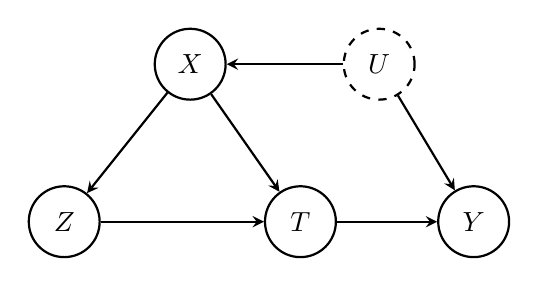
\begin{tikzpicture}[
    >=stealth,
    line width=0.8pt,
    every node/.style={circle, draw, minimum size=9mm, inner sep=0pt}
]
  %--- exact positions ---
  \node (Z) at (0,0)   {$Z$};
  \node (T) at (3,0)   {$T$};
  \node (Y) at (5.2,0) {$Y$};
  \node (X) at (1.6,2) {$X$};
  \node[dashed] (U) at (4.0,2) {$U$};  % dashed latent node

  %--- edges ---
  \draw[->] (X) -- (Z);
  \draw[->] (X) -- (T);
  \draw[->] (Z) -- (T);
  \draw[->] (T) -- (Y);
  \draw[->] (U) -- (X);
  \draw[->] (U) -- (Y);
\end{tikzpicture}
\caption{Causal DAG.}
\label{fig:causal_dag}
\end{figure}
Using Figure~\ref{fig:causal_dag} we go over the most important definitions.
\begin{itemize}[leftmargin=*, itemsep=0.25em] % compact list; remove enumitem if undesired
  \item \textbf{Parents (Children):} directly causing (caused by) a vertex \( i \to j \).
  \begin{itemize}
      \item Z is the child of X, while Y is the child of T and U.
  \end{itemize}
  \item \textbf{Ancestors (Descendants):} directly or indirectly causing (caused by) a vertex \( i \to \cdots \to j \).
  \begin{itemize}
      \item The ancestors of Y are $\{Z, X, T, U\}$, the descendants of X are $\{Z, T, Y\}$.
  \end{itemize}
  \item \textbf{Path:} an acyclic sequence of adjacent nodes
    \begin{itemize}[leftmargin=2em, itemsep=0.15em]
      \item \emph{causal path:} all arrows pointing out of \(i\) and into \(j\).
      \begin{itemize}
          \item There is a causal path from Z to Y but not causal path from T to U.
      \end{itemize}
      \item \emph{non-causal path:} some arrows going against the causal order.
      \begin{itemize}
          \item There is a non-causal path from T to U and Y to X.
      \end{itemize}
    \end{itemize}
    \item \textbf{Collider:} a vertex on a path with two incoming arrows
    \begin{itemize}
        \item T is a collider for the path $X \to T \leftarrow Z$.
    \end{itemize}
\end{itemize}

Every DAG encodes \emph{nonparametric structural equations}. In Figure~\ref{fig:causal_dag} the equations read as follow (assuming an unmeasured confounder $U$)
\begin{align*}
    Y &= f_Y(T, U, \epsilon_Y),
    \\
    T&= f_T(X, Z, \epsilon_T),
    \\
    Z &= f_Z(X, \epsilon_Z),
    \\
    X &= f_X(U, \epsilon_X).
\end{align*}

\subsection{Likelihood Factorization}
This subsection is inspired
A primary purpose of a DAG is that it encodes conditional independence. Consider vertices $V = \{1, \ldots, J\}$ corresponding to $\{X_1, \ldots, X_J\}$. For $i \in \{1, \ldots, J\}$ we define
\begin{align*}
    \mathrm{pa}(i) &= \{j: X_j \text{ is a parent of } X_i\},
    \\
    \mathrm{de}(i) &= \{j: X_j \text{ is a descendant of } X_i\},
\end{align*}
the set of indices corresponding to the parents and descendents of $X_i$. For each $i$ we have
\[
    X_i \ind X_{V \setminus \{\mathrm{pa}(i) \cup \mathrm{de}(i) \cup \{i\}\}} \mid  X_{{\mathrm{pa}(i)}} ,
\]
that is, given $i$-th parents, $X_i$ is independent of all other vertices except its own descendants. This leads to the following factorization of the joint probability (or likelihood)
\[
    \Pr(X_1, X_2, \ldots, X_J) = \Pi_{j=1}^J \Pr(X_j \mid \text{pa}(X_j)).
\]
In Figure~\ref{fig:causal_dag} this reads as
\begin{align*}
     \Pr(T, U, X, Y, Z) &= \Pr(Y \mid T, U) \Pr(T \mid X, Z) \Pr(Z \mid X) \Pr(X \mid U) \Pr(U).
\end{align*}


\subsection{D-Separation}
\begin{figure}[h!]
\centering
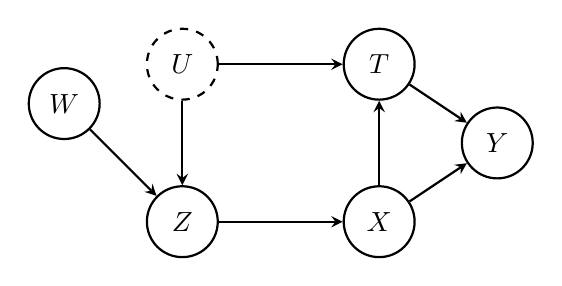
\begin{tikzpicture}[
    >=stealth,
    line width=0.8pt,
    every node/.style={circle, draw, minimum size=9mm, inner sep=0pt}
]
  % nodes (placed to match your screenshots)
  \node (W) at (-1.5,1.5) {$W$};
  \node (Z) at (0,0)      {$Z$};
  \node (X) at (2.5,0)    {$X$};
  \node (T) at (2.5,2)  {$T$};
  \node (Y) at (4,1.0)  {$Y$};
  \node[dashed] (U) at (0,2) {$U$};

  % edges
  \draw[->] (W) -- (Z);
  \draw[->] (U) -- (Z);
  \draw[->] (Z) -- (X);
  \draw[->] (X) -- (T);
  \draw[->] (T) -- (Y);
  \draw[->] (X) -- (Y);
  \draw[->] (U) -- (T);
\end{tikzpicture}
\caption{DAG for the d-separation.}
\label{fig:dsep-example}
\end{figure}

One  DAGs is that they provide information about conditional independence relationships:  \(A \perp\!\!\!\perp B \mid C\), where \(A,B,C\) are sets of vertices. The main tool for checking conditional is \emph{d-separation}:

\begin{itemize}[leftmargin=*, itemsep=0.25em]
  \item Identify all paths between \(A\) and \(B\).
  \item A path is \emph{blocked by \(C\)} if it contains
        (i) a \emph{noncollider} that is in \(C\); or
        (ii) a \emph{collider} such that neither the collider nor any of its descendants is in \(C\).
  \item \(A\) and \(B\) are \(d\)-separated by \(C\) iff \emph{every} path is blocked by \(C\). Otherwise they are  \(d\)-connected by \(C\).
\end{itemize}
If \(A\) and \(B\) are \(d\)-separated by \(C\) then \(A \perp\!\!\!\perp B \mid C\), otherwise they are not conditionally independent.

\begin{example}
    Consider Figure~\ref{fig:dsep-example}. Let \(C=\varnothing\) and ask whether \(W \perp\!\!\!\perp Y\).
    First, consider the paths between $W$ and $Y$,
    \begin{enumerate}
        \item $ W \to Z \to X \to Y$; unblocked
        \item $W \to Z \to X \to T \to Y$; unblocked
        \item $W \to Z \leftarrow U \to T \to Y$; blocked by $Z$
        \item $W \to Z \leftarrow U \to T \leftarrow X \to Y$; blocked by $Z$
    \end{enumerate}
    Since there exist unblocked paths, \(W\) and \(Y\) are \(d\)-connected and hence not marginally independent.
\end{example}

\begin{example}
    Consider Figure~\ref{fig:dsep-example}. For what $C$ do we have \(W \perp\!\!\!\perp Y \mid C\)?
    We need to find a set of vertices such that we block all paths between $W$ and $Y$. For example,
    \[
    C=\{X, T\}\quad\Rightarrow\quad
    W \perp\!\!\!\perp Y \mid X, T ,
    \]
    as now paths 1. and 2. are blocked, while paths 3. and 4. are as blocked as well ($X$ opens them, but $T$ blocks them).
    Conditioning on \(Z\) or \(T\) would open blocked collider paths
\(W \to Z \leftarrow U \cdots\) or \(\cdots U \to T \leftarrow X \cdots\). 
Conditioning just on $C = \{X\}$ would open paths 3. and 4., as $X$ is a descendant of the collider $Z$.
\end{example}
\noindent
\textbf{Remember:} We want to choose $C$ without colliders.

\subsection{Backdoor Criterion}
When can we identify the causal effect of $T$ on $Y$ given a set of variables $X$? The \emph{backdoor} criterion establishes under what conditions on $X$ we can identify the causal effect.
\begin{enumerate}
    \item No vertex in $X$ is a descendant of $T$ (no post-treatment bias),
    \item $X$ blocks all paths between $T$ and $Y$ with an incoming error into $T$.
\end{enumerate}
Under these conditions we have 
\[
    \Pr(Y(t) = y) = \sum_x \Pr(Y \mid T = t, X = x) \Pr(X = x).
\]
\begin{example}
   In Figures~\ref{fig:causal_dag} and~\ref{fig:dsep-example} controlling for the vertex $X$ is enough to identify the causal effect.
\end{example}

% --- in preamble once ---
% \usepackage{tikz}
% \usetikzlibrary{positioning}

\subsection{Frontdoor Criterion}\label{subsec:frontdoor}

\begin{figure}[h!]
\centering
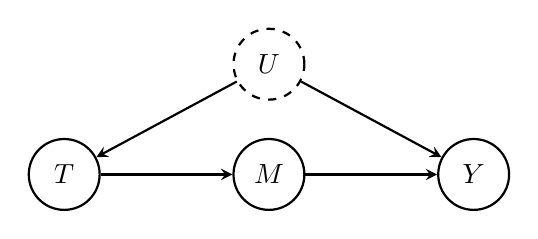
\begin{tikzpicture}[
    >=stealth,
    line width=0.8pt,
    every node/.style={circle, draw, minimum size=9mm, inner sep=0pt}
]
  % nodes
  \node (T) at (0,0)      {$T$};
  \node (M) at (2.6,0) {$M$};
  \node (Y) at (5.2,0)    {$Y$};
  \node[dashed] (U) at (2.6,1.4) {$U$};

  % edges
  \draw[->] (T) -- (M);
  \draw[->] (M) -- (Y);
  \draw[->] (U) -- (T);
  \draw[->] (U) -- (Y);
\end{tikzpicture}
\caption{Frontdoor DAG with mediator $M$ and unobserved $U$.}
\label{fig:frontdoor}
\end{figure}

When an unmeasured confounder $U$ exists, we can use a \emph{mediator} $M$ to identify the causal effect of $T$ on $Y$. This is called the \emph{frontdoor} criterion.

\begin{enumerate}
  \item $M$ intercepts all directed paths from $T$ to $Y$ (no $T\to Y$ edge bypassing $M$).
  \item No backdoor path from $T$ to $M$.
  \item All backdoor paths from $M$ to $Y$ are blocked by $T$
        (here, the only one is $M \leftarrow T \leftarrow U \to Y$, blocked by conditioning on $T$).
\end{enumerate}

Under these conditions,
\[
 \Pr\big(Y(t)=y\big)
= \sum_{m}  \Pr(M = m \mid T = t)\;\sum_{t'}  \Pr\big(Y = y \mid T = t', M = m\big)\, \Pr(T = t'),
\]
so the causal effect of $T$ on $Y$ is identified from observational data via the mediator $M$.

\subsection{Don't Condition on Colliders}

\begin{figure}[h!]
\centering
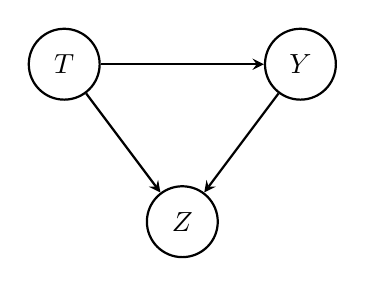
\begin{tikzpicture}[
    >=stealth,
    line width=0.8pt,
    every node/.style={circle, draw, minimum size=9mm, inner sep=0pt}
]
  % nodes
  \node (T) at (1,0)      {$T$};
  \node (Y) at (4,0)    {$Y$};
  \node (Z) at (2.5, -2) {$Z$};

  % edges
  \draw[->] (T) -- (Y);
  \draw[->] (T) -- (Z);
  \draw[->] (Y) -- (Z);
\end{tikzpicture}
\caption{$Z$ is a collider for $T$ and $Y$.}
\label{fig:collider}
\end{figure}

Consider the DAG in Figure~\ref{fig:collider}. We investigate what happens if we condition on the collider $Z$. First, observe that $Z$ is a post-treatment variable, which is often enough reason not to adjust for it. However, since $Y$ also affects $Z$, conditioning on $Z$ induces bias. The following example illustrates this. Assume the simplified relationship,
\begin{align*}
    \begin{cases}
        Z = a T + b Y + \epsilon_Z, & 
        \\
        Y = \tau T + \epsilon_Y, &
    \end{cases}
\end{align*}
where $\epsilon_Z, \epsilon_Y \iid \mathcal{N}(0, 1)$.
In this case, the $\ATE = \E[Y(1) - Y(0)] = \E[Y \mid T = 1] - \E[Y \mid T = 0] = \tau$. However, we won't identify the correct effect if we also condition on $Z$.
\medskip
\noindent
Using joint normality, conditioning on $(Z, T)$ yields
\begin{align*}
    \E[Y \mid T = t, Z = z] &= \E[Y \mid T = t] + \frac{\Cov(Y, Z \mid T = t)}{\Var(Z \mid T = t)} (z - \E[Z \mid T = t])
    \\
    &= \tau t + \frac{b}{1 + b^2} \Big(z - (a+b\tau)t\Big)
    \\
    &= \left(\tau - \frac{ab + b^2\tau}{1 + b^2}\right)t + \frac{b}{1 + b^2} z
    \\
    &= \left(\frac{\tau - ab}{1 + b^2}\right)t + \left(\frac{b}{1 + b^2}\right) z,
\end{align*}
since,
\begin{align*}
    \E[Y \mid T = t] &= \tau t,
    \\
    \Cov(Y, Z \mid T = t) &= \Cov(Y, bY \mid T = t) = b,
    \\
    \Var(Z \mid T = t) &= b^2 \Var(Y \mid T = t) + \Var(\epsilon_Y) = b^2 + 1,
    \\
    \E[Z \mid T = t] &= (a + b\tau) t.
\end{align*}

\noindent
Taking the difference
\begin{align*}
    \E[Y \mid T = 1, Z = z] - \E[Y \mid T = 0, Z = z] &= \frac{\tau - ab}{1 + b^2} \neq \tau,
\end{align*}
yields a biased effect as long as $b \neq 0$, i.e., $Y$ affects $Z$.


\subsection{Which covariates should we adjust for?}
This subsection is taken from by \citet[Chapter~16.3.3]{ding2023coursecausalinference}. We try to give a general recipe for what to adjust for to identify the causal effect of $T$ on $Y$.

\begin{figure}[h!]
\centering
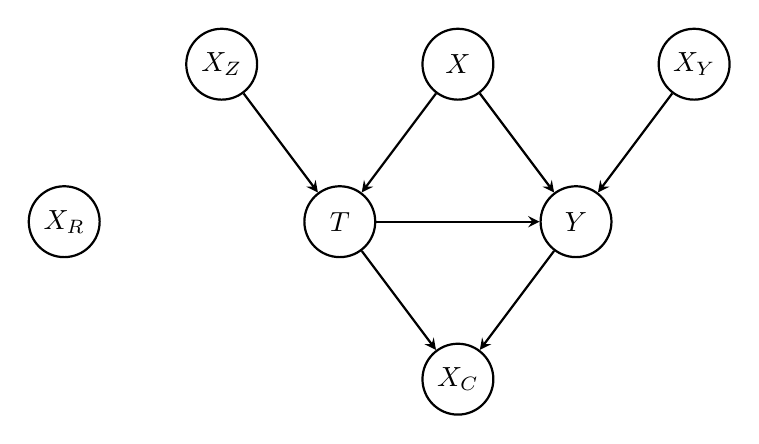
\begin{tikzpicture}[
  >=stealth, line width=0.8pt,
  every node/.style={circle, draw, minimum size=9mm, inner sep=0pt}
]
  % positions
  \node (XZ) at (-0.5,2) {$X_Z$};
  \node (X)  at (2.5,2)    {$X$};
  \node (XY) at (5.5,2)  {$X_Y$};
  \node (XR) at (-2.5,0)   {$X_R$};
  \node (T)  at (1,0)      {$T$};
  \node (Y)  at (4.0,0)    {$Y$};
  \node (XC) at (2.5,-2) {$X_C$};

  % edges
  \draw[->] (X)  -- (T);
  \draw[->] (X)  -- (Y);
  \draw[->] (XZ) -- (T);
  \draw[->] (XY) -- (Y);
  \draw[->] (T)  -- (Y);
  \draw[->] (T)  -- (XC);
  \draw[->] (Y)  -- (XC);
  % (X_R has no arrows by design)
\end{tikzpicture}
\caption{Guiding DAG for covariate adjustment.}
\label{fig:adj_which}
\end{figure}

\begin{itemize}
  \item \textbf{Adjust for $X$ (confounder).} It affects both $T$ and $Y$; conditioning on $X$ secures ignorability.
  \item \textbf{Do \emph{not} condition on $X_R$ (pure noise).} It affects neither $T$ nor $Y$; including it doesn’t bias estimates but adds variance.
  \item \textbf{Do \emph{not} condition on $X_Z$ (instrument).} It moves $T$ but not $Y$ directly; adjusting can inflate variance and, with unmeasured confounding, \emph{amplify} bias (``Z-bias''). 
  \item \textbf{Optionally adjust for $X_Y$ (outcome-only predictor).} Ignorability already holds without it, but conditioning on $X_Y$ often improves precision. 
  \item \textbf{Do \emph{not} adjust for $X_C$ (post-treatment collider).} Being affected by $T$ (and possibly $Y$), it is not a pre-treatment covariate.
\end{itemize}

\noindent\textbf{Takeaway.} If the DAG in Figure~\ref{fig:adj_which} is plausible, adjust for at least $X$ to remove bias; adding $X_Y$ can further reduce variance.  



\endgroup

\newpage

\bibliography{references}


\end{document}
